

\documentclass[
	parspace, % Add vertical space between paragraphs
	noindent, % No indentation of first lines in each paragraph
	nohyp, % No hyphenation of words
	%twoside, % Double sided format
	%draft, % Quicker draft compilation without rendering images
	%final, % Set final to hide todos
]{elteikthesis}[2023/04/10]

% The minted package is also supported for source highlighting
% See elteikthesis_minted.tex for example
%\usepackage[newfloat]{minted}

% Document's metadata
\title{Ekvivalens Python forráskód-párok generálása} % title
\date{2024} % year of defense

% Author's metadata
\author{Verebics Péter}
\degree{programtervező informatikus BSc}

% Superivsor(s)' metadata
\supervisor{Szalontai Balázs} % internal supervisor's name
\affiliation{doktorandusz} % internal supervisor's affiliation
%\extsupervisor{Külső Kornél} % external supervisor's name
%\extaffiliation{informatikai igazgató} % external supervisor's affiliation

% University's metadata
\university{Eötvös Loránd Tudományegyetem} % university's name
\faculty{Informatikai Kar} % faculty's name
\department{Programozáselmélet és Szoftvertechnológiai\\ Tanszék} % department's name
\city{Budapest} % city
\logo{elte_cimer_szines} % logo

% Add bibliography file
\addbibresource{elteikthesis.bib}

% The document
\begin{document}

% Set document language
\documentlang{hungarian}
%\documentlang{english}

% List of todos (not in the final document)
%\listoftodos[\todolabel]

% Title page (mandatory)
\maketitle
% Topic declaration page (mandatory) - can also be attached instead
%\includepdf{temabejelento.pdf}

% Table of contents (mandatory)
\tableofcontents
\cleardoublepage

% Main content
\chapter{Bevezetés}
\label{ch:intro}

Szakdolgozatom témája Python forráskódok átalakítása, és ezen átalakítások szemléltetése.
A motiváció az átalakítások mögött egy olyan adathalmaz generálása amiben ekvivalens és nem
ekvivalens 
forráskód-párok egyaránt szerepelnek. Egy ilyen adathalmazt felhasználhatunk egy mélytanuló
neuronháló tanítására,
ami forráskód-párok ekvivalenciáját dönti el.

Az ekvivalencia eldöntése fontos feladat, mivel egyre több, kódokat gépi tanulással refaktoráló
eszköz létezik.
Ezek az eszközök egy kódot változtatva sokszor a kód jelentését is megváltoztatják.
Egy ekivalenciát eldöntő neuronháló képes lenne kiszűrni az ilyen eszközök által generált
rossz eredményeket, javítva az eszközök hatékonyságán.
Tehát ekvivalens és nem ekvivalens kódokat generálva felépíthetünk egy adathalmazt, ami
ekvivalenciával felcímkézett kódpárokat tartalmaz, és alkalmas egy fent leírt neuronháló
tanítására.

Az általam implementált átalakítások absztrakt szintaxisfák (AST-k) módosításával működnek.
Egy forráskód fordítása alatt a szemantikus elemző előállítja a kód AST-jét,
ami a kódot egy fa adatstruktúrával reprezentálja.
Az AST-nek a szemantikus elemzésben van szerepe,
de használhatjuk kódok átalakítására is, mivel visszaakítható forráskóddá.

Az általam megvalósított átalakítások a Python \emph{ast} modult \cite{pythonAST} használják,
amely része a Python standard könyvtárának.

\pagebreak

Az átalakításokat szabályok végzik. Átalakításkor 
a Python kódból létrehozott AST-n végrehajthatunk egy szabályt.
A szabály megváltoztatja az AST-t, amit ha visszaalakítunk kóddá,
egy megváltozott Python kódot kapunk.

A szakdolgozatomban ekvivalens és nem ekvivalens szabályokat is definiálok.
Egy szabály akkor tekinthető ekvivalensnek, ha a kód szemantikáját nem változtatja meg.
Például a Python-ban is teljesül a valós számok körében a szorzás kommutatív tulajdonsága.
Tehát, ha egy Python kódban két szám szorzásánál a bal és jobb operandust megcseréljük,
akkor a szorzás eredménye nem változik, vagyis ez az átalakítás ekvivalens.
Ez a példa természetesen nagyon egyszerű, a szakdolgozatomban összetettebb átalakítások
is szerepelnek.

Az adathalmazban az ekvivalens kódok generálásához saját szabályok mellett
a \emph{ruff} Python linter és formatter szabályait is felhasználtam.
A \emph{ruff} már létező Python lintereket implementál Rust programozási nyelven,
így sok más Python refaktoráló eszköz szabályait is képes elvégezni,
amelyek tökéletesek az általam implementált szabályok kiegészítésére.

A szakdolgozatom következő fejezeteiben az adathalmaz generálására és az átalakítások
szemléltetésére alkalmas szoftver használatát és működését részletezem.

\cleardoublepage

\chapter{Felhasználói dokumentáció}
\label{ch:user}

A szoftver két felhasználói felülettel rendelkezik.
Az egyik egy parancssoros (CLI) program az adathalmaz generálásához,
a másik egy grafikus (GUI) alkalmazás az átalakítások szemléltetéséhez és az adathalmaz böngészéséhez.
Mindkét alkalmazás felületének nyelve angol.

\section{Futtatási környezet}

A szoftver egy Python 3.10-es vagy újabb verziójú Python interpreterrel futtatható.
Futtatás előtt a szoftver a függőségeit installálni kell a \emph{pip} csomagkezelővel.
Ezt a legegyszerűbben a szoftver forráskódjának könyvtárból tehetjük,
a következő parancs kiadásával:

\begin{lstlisting}[language=bash, numbers=none]
	$ pip install --editable .
\end{lstlisting}

\section{Adatbázis beállítása}

Az adathalmaz generálásához szüksége van egy \emph{mongodb} adatbázis kliensre \cite{installMongodb}.
Az adatbázis kiszűri a kódpárok generálása közben a duplikált kódokat
és az adatok lekérdezését is megkönnyíti.

Az adatbázis elérést a forrás könyvtárában a \emph{config/default.ini} útvonal alatt található
konfigfájlban lehet beállítani.
Egy adatbázist három paraméter határoz meg: \emph{host}, \emph{port}, \emph{database} (az adatbázis neve).
Ha szükséges a konfigfájl alapértékeit átírhatjuk.

\section{Adathalmazt generáló CLI}

Ezzel a CLI alkalmazással van lehetőségünk az adathalmaz generálására egy
adott csv fájlban található kódokból vagy egy könyvtárban taláható forrásfájlokból.
Adathalmazt a következő paranccsal generálhatunk:

\begin{lstlisting}[language=bash, numbers=none]
	$ python -m source.persistor <mode> <path>
\end{lstlisting}

A parancs paraméterei a következők:

\begin{enumerate}
	\item\label{step:first} \emph{mode} - az adatok forrásának típusa,
	lehetséges értékek:
	\begin{itemize}
		\item \emph{csv} - csv fájlból olvassa a forrásfájlok tartalmát
		\item \emph{dir} - könyvtárból rekurzívan olvassa a forrásfájlokat
	\end{itemize}
	\item \emph{path} - az adatok forrásának elérési útvonala
\end{enumerate}

Ha megadtuk a parancsot a program megpróbálja a forráskódok olvasását,
ha az input nem megfelelő leáll.

Futás közben a program a kiírja az éppen feldolgozott forráskóddal kapcsolatos információkat,
például a kódon végzett átalakítások számát és azt, hogy el tudta-e menteni az átalakítások eredményeit.

\begin{figure}[H]
	\centering
	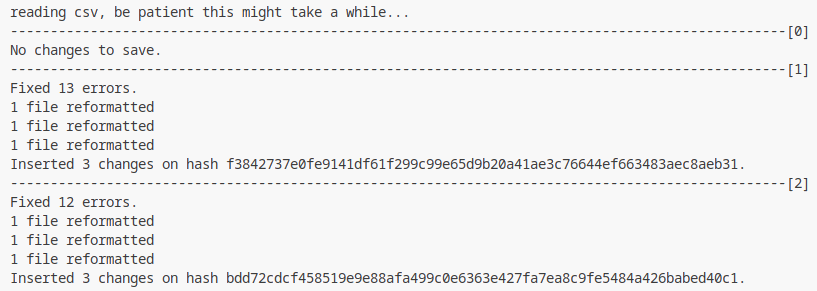
\includegraphics[width=0.9\textwidth,frame]{images/screenshots/log.png}
	\caption{A CLI alkalmazás futás közben}
\end{figure}

Ha a program végigolvasta a csv fájlt vagy a könyvtárban található forrásfájlokat leáll.
Miután a program leállt a forráskód-párok már az adatbázisban vannak.

A \emph{mongoexport} eszköz segítségével
az adatbázisból a forráskód-párokat egy csv fájlba exportálhatjuk.

\section{Átalakításokat szemléltető GUI}

Ez a GUI alkamazás szemlélteti az átalakításokat.
Kipróbálhatunk vele egy vagy több átalakító szabályt,
vizualizálhatjuk kódok absztrakt szintaxis fáját,
és az adatbázisba bekerült átalakítások eredményét is megnézhetjük.

\subsection{Alkalmazás indítása}

Az alkalmazás a forrás könyvtárából indítható a következő paranccsal:

\begin{lstlisting}[language=bash, numbers=none]
	$ python -m source
\end{lstlisting}

A parancs kiadása után felugró ablakban beállíhatjuk az adatbázis kapcsolathoz szükséges paramétereket:
a \emph{host}, \emph{port} illetve \emph{database} értékeit.
A \emph{Connect} gombra kattintva az alkalmazás adatbáziseléréssel indul,
ha a megadott adatbázishoz 10 másodperc alatt kapcsolódni tud, különben adatbáziselérés nélkül.
Adatbáziselérés nélkül a \emph{Launch Now} gombbal indíthatjuk az alkalmazást.

\begin{figure}[H]
	\centering
	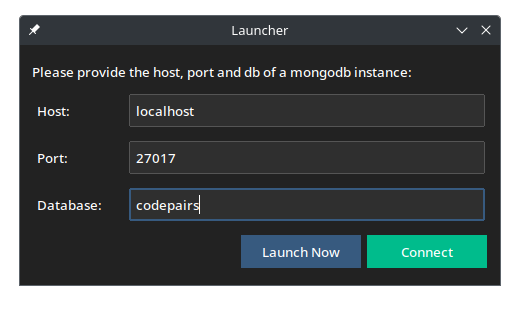
\includegraphics[width=0.5\textwidth]{images/screenshots/launcher.png}
	\caption{Az alkalmazást indító ablak}
\end{figure}

\subsection{Alkalmazás felülete}

Az alkalmazás felülete funkciók szerint két fő nézetre osztható,
a refaktoráló és az adatbázis-böngésző nézetre.
A menü gombjai és az állapotsor szövegei a két fő nézeten kívül helyezkednek el.

A refaktoráló nézetben (\emph{Refactor} tab) egy kódon
ekvivalensen és nem ekvivalensen átalakító szabályokat próbálhatunk ki, és elmenthetjük
a szabályok által végzett átalakítások eredményeit.

Az adatbázis-böngésző (\emph{Database} tab) nézetben az adatbázisba bekerült kódpárokat tekinthetjük meg.

\subsection{Refaktoráló nézet}

Indítás után a felhasználót a refaktoráló nézet fogadja.
Egy Python forráskód átalakításához a kódot begépelhetjük a \emph{Source Code} szöveges input mezőbe,
vagy egy \emph{.py} fájlból is betölthetjük a menüben látható \emph{Open File} gombra kattintva.

\begin{figure}[H]
	\centering
	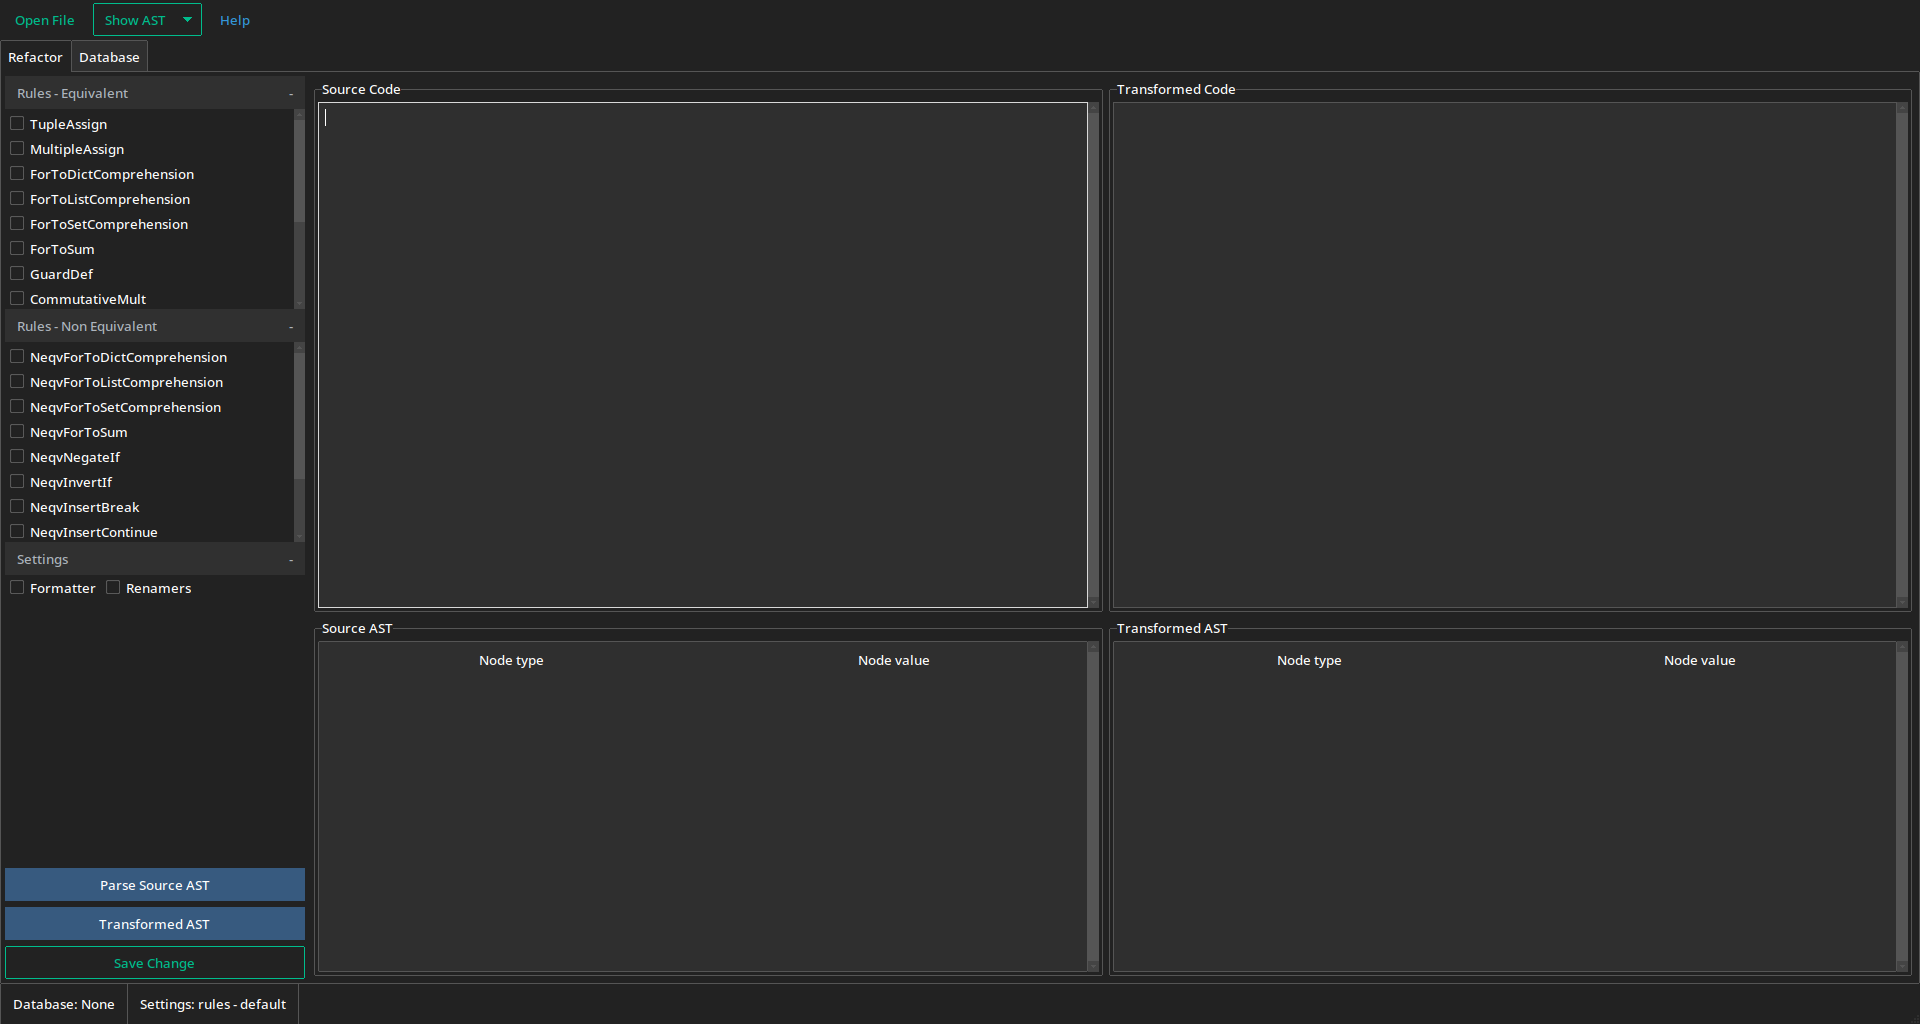
\includegraphics[width=0.9\textwidth]{images/screenshots/refactor_tab_1.png}
	\caption{Refaktoráló nézet az indítás után}
\end{figure}

Az átalakítás előtt a begépelt vagy betöltött forráskódból létre kell hozni egy AST-t
az elemező (parser) futtatásával,
ezt a \emph{Parse Source AST} gombbal tehetjük meg. Ha a megadott forráskódban szintaxis hiba található, 
vagy valami egyéb okból kifolyólag nem elemezhető, akkor az alkalmazás ezt jelzi egy felugró 
párbeszéd-ablakkal. Akkor is jelez ha parse-olás nélkül klikkelünk az átalakító gombra.

\begin{figure}[H]
	\centering
	\subcaptionbox{elemzési hiba esetén}{
		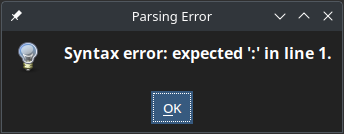
\includegraphics[width=0.5\linewidth]{images/screenshots/syntax_error.png}}
	\hspace{5pt}
	\subcaptionbox{hiányzó AST esetén}{
		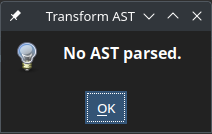
\includegraphics[width=0.31\linewidth]{images/screenshots/no_ast_parsed.png}}
	\caption{Hibákat jelző párbeszéd-ablakok}
\end{figure}

Sikeres elemzés után az AST felépítését a \emph{Source AST} fa-nézeten láthatjuk, 
az első oszlopban a csúcs típusa, a második oszlopban a csúcs szintaxis fájából generált kód látható. 

Elemzés után a fát átalakíthatjuk a \emph{Transform AST} gombra kattintva, 
ekkor az átalakított fa megjelenik a bal oldali \emph{Transformed AST} fa-nézeten,
az átalakított fából generált kód pedig a \emph{Transformed Code} readonly szövegdobozban.

\begin{figure}[H]
	\centering
	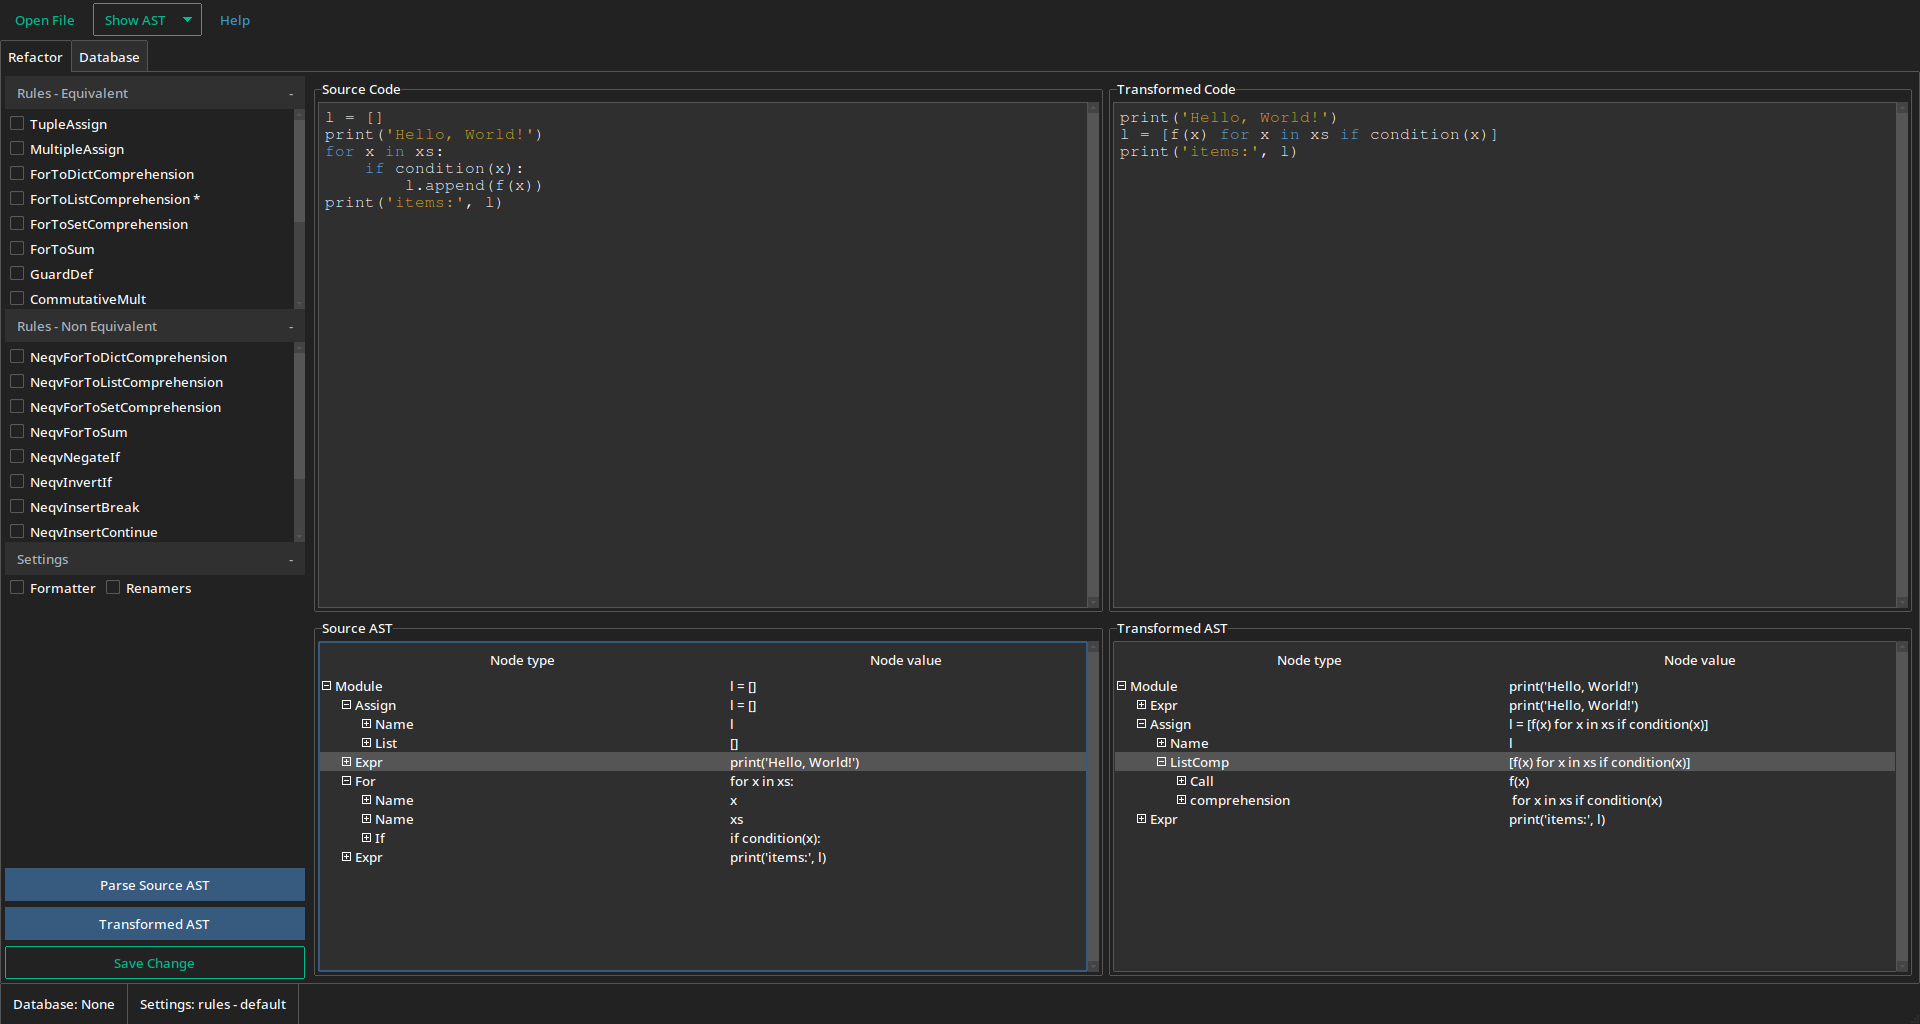
\includegraphics[width=0.9\textwidth]{images/screenshots/refactor_tab_2.png}
	\caption{Példa egy átalakítás eredményére}
\end{figure}

Az alkalmazásba összesen 28 átalakító szabály van, ezek közül 16 ekvivalens és 12 nem ekvivalens
eredményt állít elő.
Az alkalmazás indításakor az összes ekvivalens szabály ki van választva,
ez az alkalmazás alapbeállítása amit a \emph{'rules - default'} felirat jelez az állapotsorban.

Lehetőségünk van általunk választott szabályok alkalmazására is.
A szabályok listája a bal oldali panelen látható. Minden szabály előtt van egy checkbox
amivel a szabályt kiválaszthatjuk. Lehetőségünk van egy vagy több szabály kiválasztására is,
így könnyen tesztelhetjük egy szabály működését is.
Ha vannak kiválasztott szabályok azt a \emph{'rules - custom'} felirat jelzi az állapotsorban.

Átalakításkor a szabályok a bal oldali panelen látható sorrendben, fentről lefele kerülnek végrehajtásra.
A panelen a szabályokon kívül található még két checkbox is,
ezekkel a \emph{ruff} formatter és az átnevező szabályok alkalmazását tudjuk beállítani.

Miután átalakítottunk egy forráskódot kimenthetjük az átalakítás eredményét az adatbázisba
(ha van adatbázis kapcsolat).
Ezt a refaktoráló nézet bal alsó sarkában elhelyezkedő \emph{'Save Change'} gombra kattintva tehetjük.
Ha az átalakítást nem lehet elmenteni azt az alkalmazás párbeszéd-ablakban jelzi.

\subsection{AST-k vizualizálása fagráffal}

Az alkalmazás fagráfként is tud AST-ket vizualizálni.
Az általunk megadott vagy átalakított kód AST-jének fagráfját a menüben látható
\emph{Show AST} lenyíló menügombbal vizualizálhatjuk.
A gombra klikkelve két opció közül választhatunk:
a \emph{Source} gomb az általunk megadott kód, a \emph{Transformed} gomb pedig az átalakított kód
AST-jét vizualizálja, ha ezek léteznek.
Az alkalmazás az elkészült fagráf ábráját egy felugró ablakban nyitja meg.
Az alábbi ábrán például a \emph{helloworld} Python kódjának AST-jét láthatjuk:

\begin{figure}[H]
	\centering
	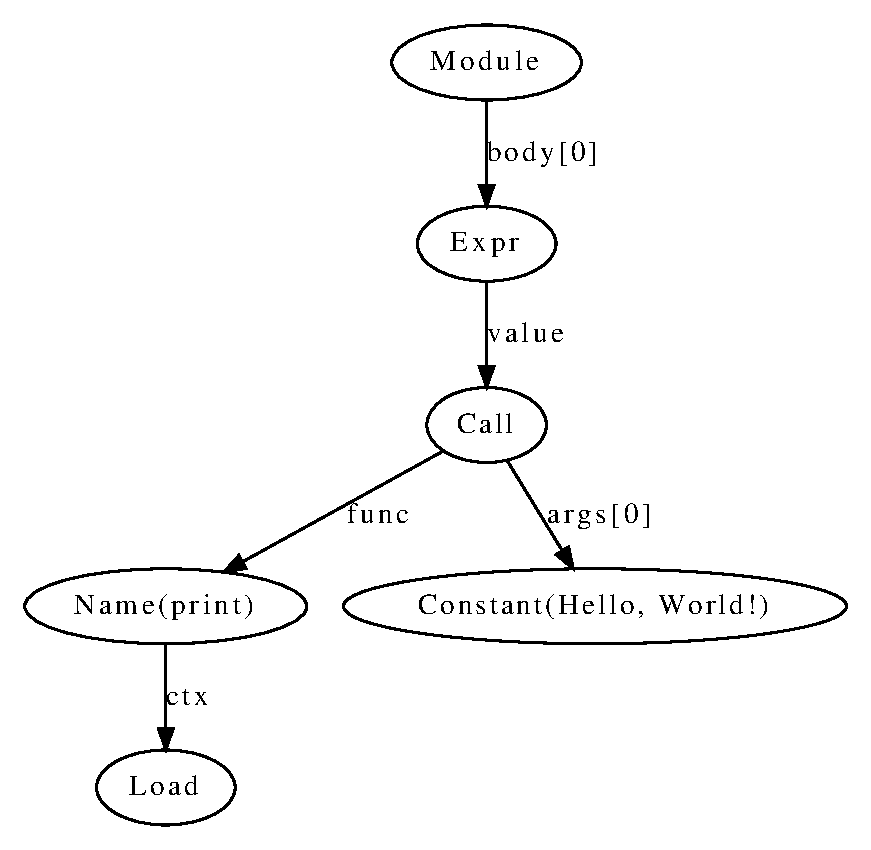
\includegraphics[width=0.6\textwidth]{images/figs/ast_graph.eps}
	\caption{A \emph{helloworld} program AST-je}
\end{figure}

\subsection{Adatbázis-böngésző nézet}

Ebben a nézetben megtekinthetjük az adatbázisba bekerült forráskód-párokat.
A nézet csak akkor jön létre ha az alkalmazásnak van adatbázis elérése,
ha nincs azt a nézeten a \emph{"No database connection."} felirat jelzi.
A nézet feladata a forráskód-párok listázása és a párba állított forráskódok
különbségeinek megjelenítése.

A különbségeket két forráskód között könnyen vizualizálhatjuk egy diffel,
azaz olyan szövegösszehasonlító programmal, ami szöveg közti a különbségek
listáját állítja elő.
A különbségeket a forráskód-párokban ezzel a módszerrel vizualizálom.

\begin{figure}[H]
	\centering
	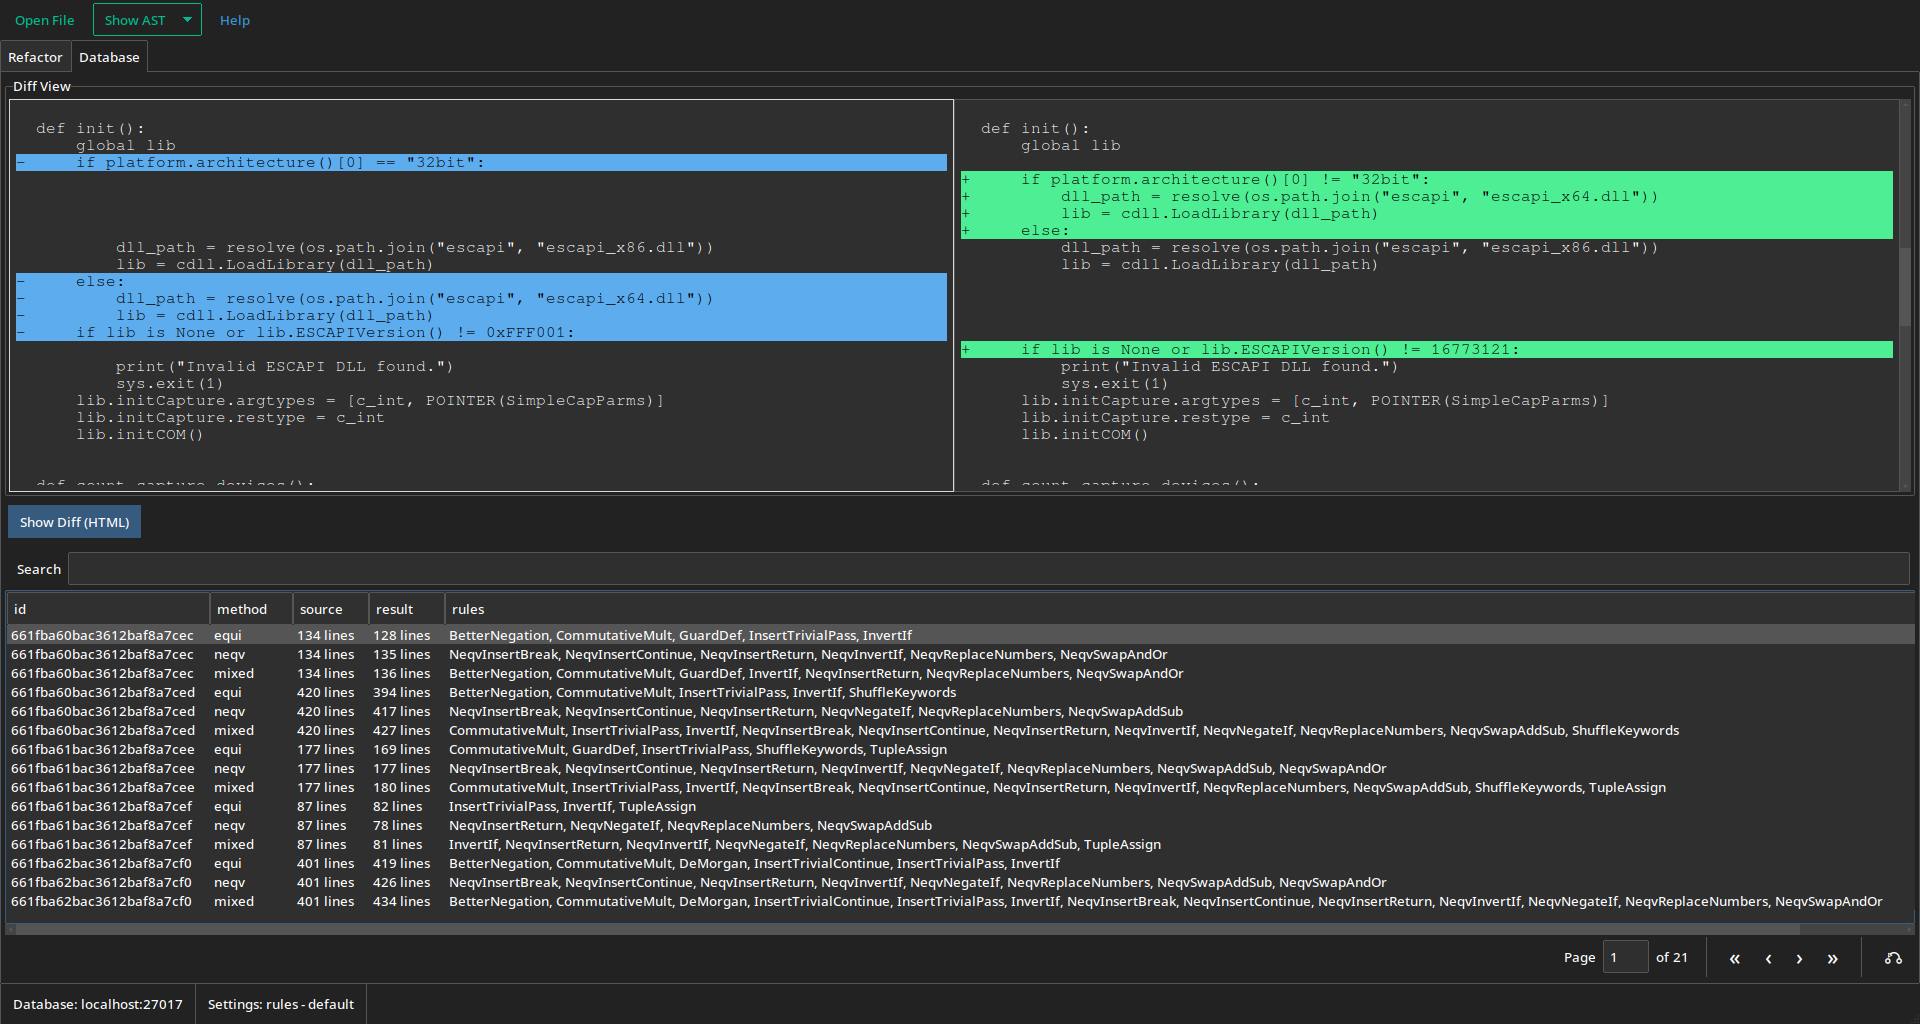
\includegraphics[width=0.9\textwidth]{images/screenshots/database_tab.png}
	\caption{Adatbázis-böngésző nézet}
\end{figure}

A nézet tetején találhatók a diffeket megjelenítő szövegdobozok, ezek alatt
egy táblázat látható, soraiban az adatbázisba bekerült forráskód-párokkal.
A táblázat soraiban található adatok sémáját a \ref{tab:schema}. táblázat írja le.

\begin{table}[H]
	\centering
	\begin{tabular}{ | m{0.15\textwidth} | m{0.75\textwidth} | }
		\hline
		\textbf{Oszlop} & \textbf{Magyarázat} \\
		\hline \hline

		\emph{id}
		& az eredeti forrráskód azonosítóját tartalmazó oszlop \\
		\hline
		
		\emph{method}
		& az átalakításra használt módszerre utaló oszlop
		
		(például a szabályhalmazra) \\
		\hline
		
		\emph{source}
		& az eredeti forráskód sorainak számát tartalmazó oszlop \\
		\hline
		
		\emph{result}
		& az átalakított forráskód sorainak számát tartalmazó oszlop \\
		\hline
		
		\emph{rules}
		& az átalakításnál alkalmazott szabályok listája (szöveg) \\
		\hline
	\end{tabular}
	\caption{Adatbázis-böngésző nézet táblázatának oszlopai}
	\label{tab:schema}
\end{table}

Ha a táblázat egy sorára, vagyis egy forráskód-párra klikkelünk
akkor a diff nézetben megjelennek az eredeti (bal oldali) és az átakított (jobb oldali)
kód közti különbségek.

A táblázat feletti keresőt használathatjuk a forráskód-párok böngészéséhez.
A kereső az összes sorban és oszlopban szereplő adatok közt keres.
Például megkereshetjük, hogy az adatbázisban mely forráskódokon kerültek
for ciklussal kapcsolatos átalakítások alkalmazásra.

\cleardoublepage

\chapter{Fejlesztői dokumentáció}
\label{ch:impl}

\textbf{TODO: intro}

\section{Csomagok}

A szoftver forráskódja több csomagban és modulban található.
A forrráskód jelentős része öt fő csomagba van szerveze,
ezek az alábbi táblázatban láthatók.

\begin{table}[H]
	\centering
	\begin{tabular}{ | m{0.25\textwidth} | m{0.65\textwidth} | }
		\hline
		\textbf{Csomag} & \textbf{Rövid leírás} \\
		\hline \hline
		\emph{app} & GUI alkalmazás csomagja \\
		\hline
		\emph{client} & adatbázis kliens \\
		\hline
		\emph{model} & adatok modelezése és mentése \\
		\hline
		\emph{tests} & egység és egyéb tesztek \\
		\hline
		\emph{transformations} & átalakítások forráskódja és API az átalakításokhoz \\
		\hline
	\end{tabular}
	\caption{A szoftver fő csomagjai}
	\label{tab:packages}
\end{table}

Minden csomag a szoftver egy jól elkülöníthető részét vagy funkcióját valósítja meg.
A fő csomagok (a \emph{tests} csomag kivételével) nem tartalmaznak "futtatható" fájlokat,
a belépési pontok külön modulokba vannak szervezve.

\section{\emph{app} csomag}

Az \emph{app} csomag feladata az átalakításokat szemléltető GUI-s alkalmazás megvalósítása.
Az alkalmazás architektúrája model-nézet-kontroller (MVC) szerű.
Egy nézet rendelkezik egy kontrollerrel és a kontroller pedig egy modellel.

A nézet feladata a GUI definiálása és frissítése,
a model feladata az adatelérés vagy az alkalmazás állapotának modelezése.
A kontroller ezt a két réteget köti össze,
így a nézet nem függ a modeltől és a model sem a nézettől.

Tegyük fel, hogy a nézeten történik egy GUI esemény, például a felhasználó egy gombra klikkel,
aminek az eseménykezelője a model használatát igényli.
Ekkor az eseménykezelő a nézet kontrollerének továbbítja a megfelelő adatokat.
A kontroller használja a modelt, majd a nézetet direk vagy indirekt módon frissíti.
Direkt módon frissíti, ha a modeltől kapott adatokat a nézetnek továbbítja,
ha pedig egy eseményt vált ki a modelben aminek hatására a nézet frissül akkor indirekt frissíti.
Ezt a működést az alábbi ábrán láthatjuk.

\begin{figure}[H]
	\centering
	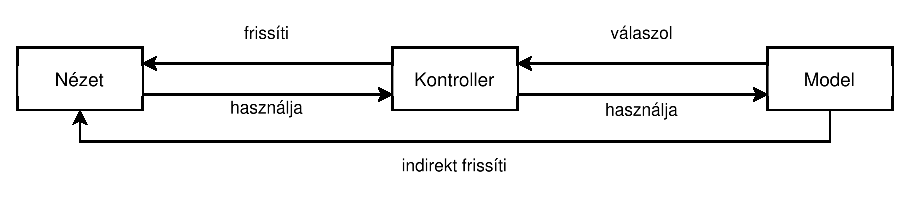
\includegraphics[width=0.9\textwidth]{images/figs/mvc.eps}
	\caption{Egy esemény kezelése az MVC architektúrában}
\end{figure}

\subsection{Állapotmodel}

Az alkalmazásban kétféle model különböztethető meg: az állapot és adatelérési modelek.
Az alkalmazás állapotmodelje az \emph{app.appstate} modulban található.
Az adatelérési modelek nem az alkalmazás csomagjában vannak definiálva mivel 
a szoftver más rétegeinek is szüksége van ezekre.

Az állapotmodel az \emph{observer} tervezési mintát használja a nézetek frissítésére
és az \emph{AppState} osztályban van definiálva.
Az \emph{AppState} osztály az \emph{Observable} osztályból származik,
ezért rendelkezik megfigyelők (\emph{observers}) egy listájával,
ami esemény-eseménykezelő párok listája.

Ha a nézet egy komponenesét az állapotmodel változásának hatására akarjuk frissíteni,
akkor azt az eseménykezelőt, ami frissíti, hozzárendelhetjük az állapotmodel egy eseményéhez.

Hozzárendelni egy eseménykezelőt egy eseményhez az \emph{Observable} osztály \emph{attach}
metódusával lehet.
Ha az adott eseményt kiváltja egy változás a modelben, akkor a model értesíti a nézeteket,
vagyis az \emph{observers}-ben az eseményéhez rendelt eseménykezelőket meghívja,
a frissítéshez szükséges adatokat paraméterként továbbítva.

\begin{figure}[H]
	\centering
	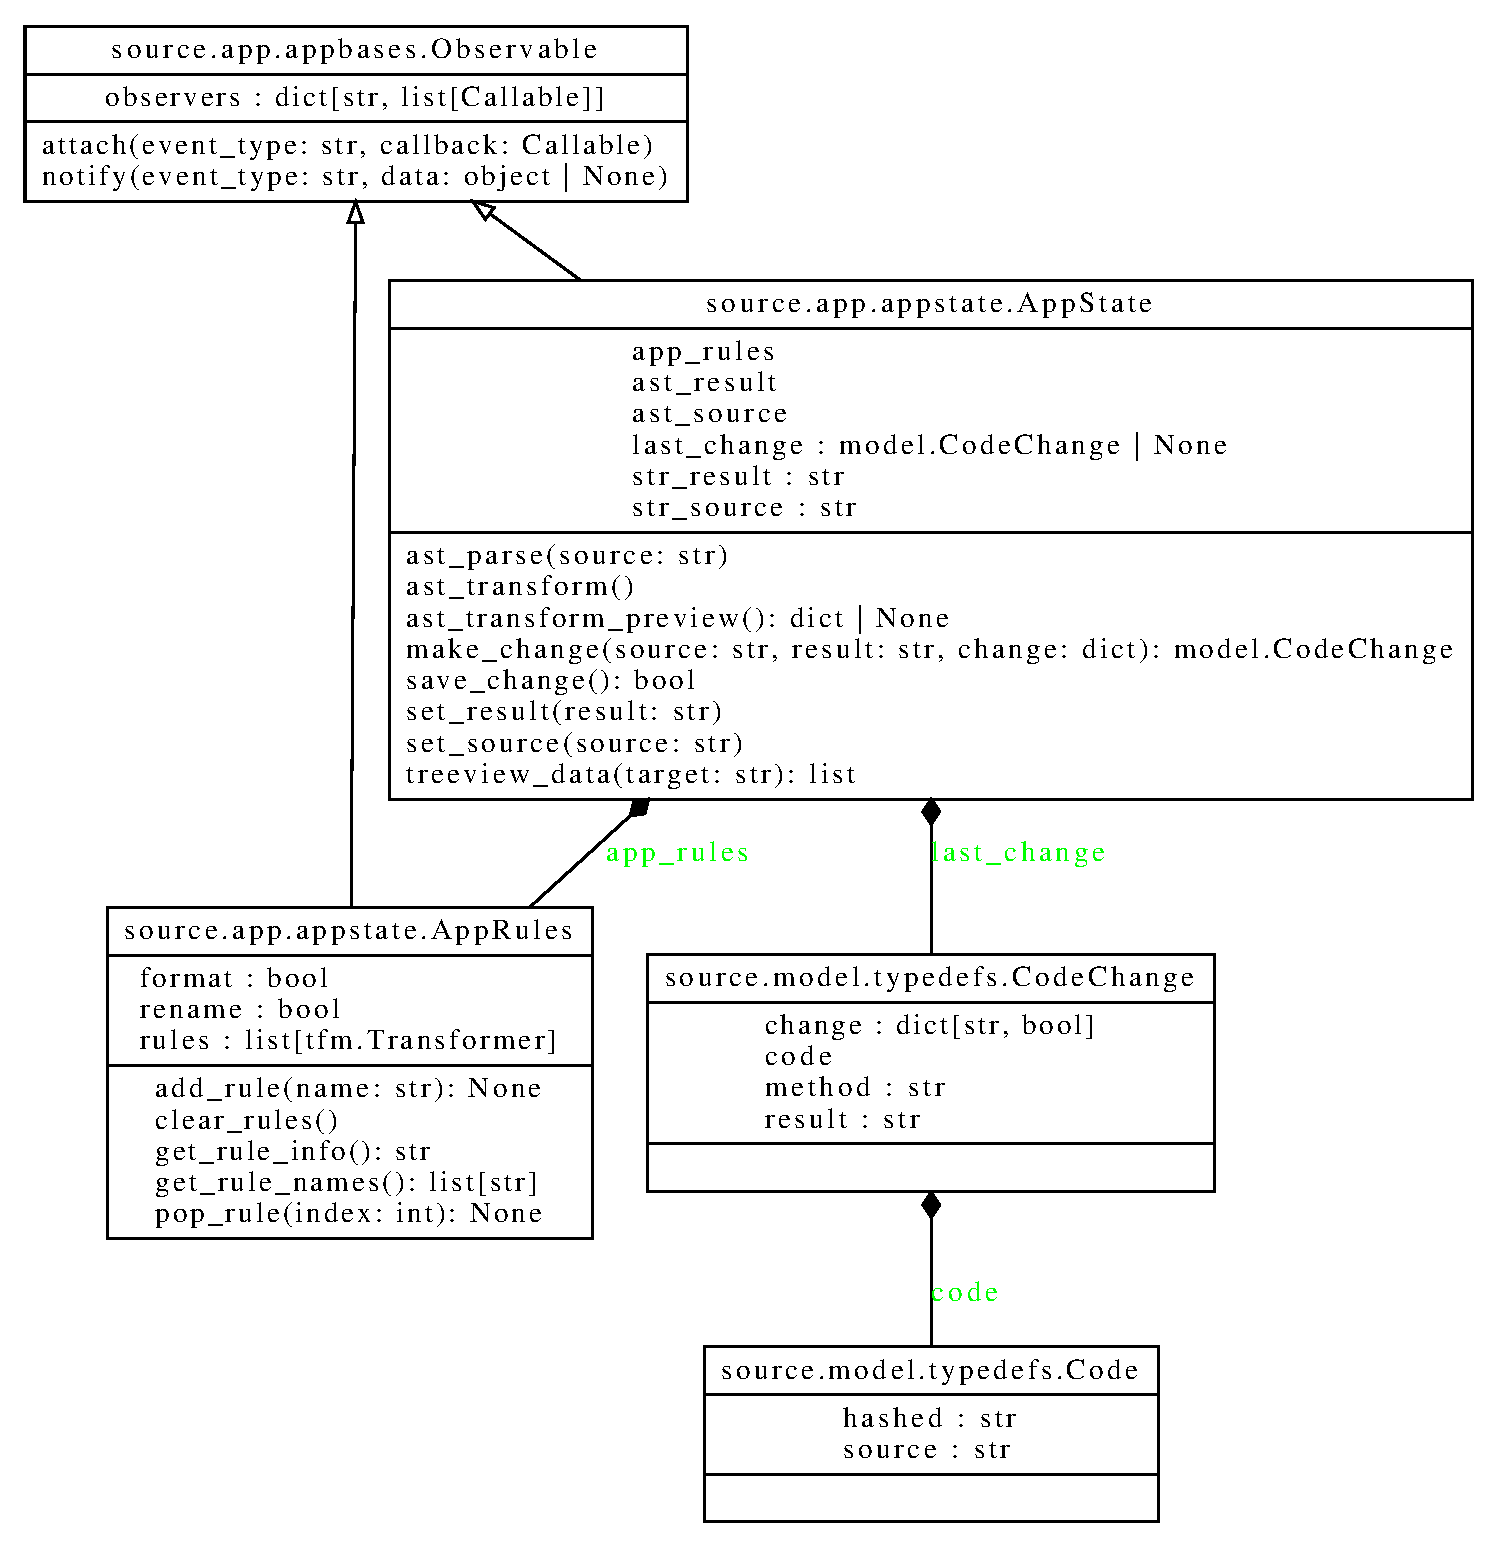
\includegraphics[width=0.9\textwidth]{images/uml/AppState.eps}
	\caption{Állapotmodel UML diagramja}
\end{figure}

\pagebreak

A felhasználói felület (View-réteg) kódja a \emph{app.views} csomagban található,
a Python-ban alapból megtalálható \emph{tkinter} könyvtárt használja, amit az 
erre építő \emph{ttkbootstrap} könyvtárral egészít ki.

A kontrollerek feladata a kommunikáció a modelek és nézetek között.
Csak a felhasználói felület két fő nézete
a \emph{RefactorTab} és a \emph{DatabaseTab} 
rendelkeznek saját kontrollerekkel.
\cleardoublepage

\chapter{Összegzés}
\label{ch:sum}

Szakdolgozatomban egy Python kódok átalakítására alkalmas szoftvert mutattam be.
Az átalakításokat végző szoftver segítségével GitHub-ról bányászott kódokból generáltam
ekvivalens és nem ekvivalens forráskód-párokat tartalmazó adathalmazt.
Az adathalmazt egy forráskód-pár ekvivalenciáját eldöntő mélytanuló neuronháló tanítására használhatjuk.

Az átalakítások szemléltetésére grafikus felhasználói felületű desktop alkalmazást is készítettem,
amivel a felhasználó kipróbálhatja az átalakításokat.

A szoftver forráskódja többnyire objektum orientált,
a megvalósítás során a bővíthetőségre törekedtem.
A jövőben a szoftvert több rétegét is érdemes lehet bővíteni,
például a meglévő interfészeket használva új átalakításokat adhatunk a szoftverhez és
a GUI alkalmazás nézeteit is könnyen lecserélhetjük az MVC architektúrának köszönhetően.

Érdemes lehet változtatni az adathalmaz generálásán is. 
A szabály alapú AST-szintű átalakítások nem tudnak nagy szintaktikai változtatásokat végrehajtani,
így a bemeneti és az átalakított kódok közötti különbség sokszor kicsi.
Ezért a neuronhálót tanító adathalmazt érdemes lehet kiegészíteni egy létező,
szemantikusan ekvivalens, de szintaktikailag különböző kódokat 
tartalmazó adathalmazzal és az azon végzett átalakításokkal (pl. project-codenet).

\cleardoublepage

% Acknowledgements (optional) - in case your thesis received funding or would like to express special thanks to someone
\chapter*{\acklabel}
\addcontentsline{toc}{chapter}{\acklabel}
% Amennyiben a szakdolgozati / diplomamunka projekted
% pénzügyi támogatást kapott egy projektből vagy az egyetemtől,
% jellemzően kötelező feltüntetni a dolgozatban is.
% A dolgozat elkészítéséhez segítséget nyújtó oktatók, hallgatótársak, kollégák felé
% is nyilvánítható külön köszönet.
TODO: Tamás köszönetnyilvánítás

% Appendices (optional) - useful for detailed information in long tables, many and/or large figures, etc.
\appendix
%\chapter{Kiértékelés eredményei}
\label{appx:simulation}

TODO: kiértékelés eredményei

%\cleardoublepage

% Bibliography (mandatory)
\phantomsection
\addcontentsline{toc}{chapter}{\biblabel}
\printbibliography[title=\biblabel]
\cleardoublepage

% List of figures (optional) - useful over 3-5 figures
\phantomsection
\addcontentsline{toc}{chapter}{\lstfigurelabel}
\listoffigures
\cleardoublepage

% List of tables (optional) - useful over 3-5 tables
\phantomsection
\addcontentsline{toc}{chapter}{\lsttablelabel}
\listoftables
\cleardoublepage

% List of algorithms (optional) - useful over 3-5 algorithms
%\phantomsection
%\addcontentsline{toc}{chapter}{\lstalgorithmlabel}
%\listofalgorithms
%\cleardoublepage

% List of codes (optional) - useful over 3-5 code samples
\phantomsection
\addcontentsline{toc}{chapter}{\lstcodelabel}
\lstlistoflistings
\cleardoublepage

% List of symbols (optional)
%\printnomenclature

\end{document}
